% Options for packages loaded elsewhere
\PassOptionsToPackage{unicode}{hyperref}
\PassOptionsToPackage{hyphens}{url}
%
\documentclass[
]{article}
\usepackage{lmodern}
\usepackage{amssymb,amsmath}
\usepackage{ifxetex,ifluatex}
\ifnum 0\ifxetex 1\fi\ifluatex 1\fi=0 % if pdftex
  \usepackage[T1]{fontenc}
  \usepackage[utf8]{inputenc}
  \usepackage{textcomp} % provide euro and other symbols
\else % if luatex or xetex
  \usepackage{unicode-math}
  \defaultfontfeatures{Scale=MatchLowercase}
  \defaultfontfeatures[\rmfamily]{Ligatures=TeX,Scale=1}
\fi
% Use upquote if available, for straight quotes in verbatim environments
\IfFileExists{upquote.sty}{\usepackage{upquote}}{}
\IfFileExists{microtype.sty}{% use microtype if available
  \usepackage[]{microtype}
  \UseMicrotypeSet[protrusion]{basicmath} % disable protrusion for tt fonts
}{}
\makeatletter
\@ifundefined{KOMAClassName}{% if non-KOMA class
  \IfFileExists{parskip.sty}{%
    \usepackage{parskip}
  }{% else
    \setlength{\parindent}{0pt}
    \setlength{\parskip}{6pt plus 2pt minus 1pt}}
}{% if KOMA class
  \KOMAoptions{parskip=half}}
\makeatother
\usepackage{xcolor}
\IfFileExists{xurl.sty}{\usepackage{xurl}}{} % add URL line breaks if available
\IfFileExists{bookmark.sty}{\usepackage{bookmark}}{\usepackage{hyperref}}
\hypersetup{
  pdftitle={ECON 753 Problem Set 1},
  pdfauthor={Jesús Lara Jáuregui},
  hidelinks,
  pdfcreator={LaTeX via pandoc}}
\urlstyle{same} % disable monospaced font for URLs
\usepackage[margin=1in]{geometry}
\usepackage{color}
\usepackage{fancyvrb}
\newcommand{\VerbBar}{|}
\newcommand{\VERB}{\Verb[commandchars=\\\{\}]}
\DefineVerbatimEnvironment{Highlighting}{Verbatim}{commandchars=\\\{\}}
% Add ',fontsize=\small' for more characters per line
\usepackage{framed}
\definecolor{shadecolor}{RGB}{248,248,248}
\newenvironment{Shaded}{\begin{snugshade}}{\end{snugshade}}
\newcommand{\AlertTok}[1]{\textcolor[rgb]{0.94,0.16,0.16}{#1}}
\newcommand{\AnnotationTok}[1]{\textcolor[rgb]{0.56,0.35,0.01}{\textbf{\textit{#1}}}}
\newcommand{\AttributeTok}[1]{\textcolor[rgb]{0.77,0.63,0.00}{#1}}
\newcommand{\BaseNTok}[1]{\textcolor[rgb]{0.00,0.00,0.81}{#1}}
\newcommand{\BuiltInTok}[1]{#1}
\newcommand{\CharTok}[1]{\textcolor[rgb]{0.31,0.60,0.02}{#1}}
\newcommand{\CommentTok}[1]{\textcolor[rgb]{0.56,0.35,0.01}{\textit{#1}}}
\newcommand{\CommentVarTok}[1]{\textcolor[rgb]{0.56,0.35,0.01}{\textbf{\textit{#1}}}}
\newcommand{\ConstantTok}[1]{\textcolor[rgb]{0.00,0.00,0.00}{#1}}
\newcommand{\ControlFlowTok}[1]{\textcolor[rgb]{0.13,0.29,0.53}{\textbf{#1}}}
\newcommand{\DataTypeTok}[1]{\textcolor[rgb]{0.13,0.29,0.53}{#1}}
\newcommand{\DecValTok}[1]{\textcolor[rgb]{0.00,0.00,0.81}{#1}}
\newcommand{\DocumentationTok}[1]{\textcolor[rgb]{0.56,0.35,0.01}{\textbf{\textit{#1}}}}
\newcommand{\ErrorTok}[1]{\textcolor[rgb]{0.64,0.00,0.00}{\textbf{#1}}}
\newcommand{\ExtensionTok}[1]{#1}
\newcommand{\FloatTok}[1]{\textcolor[rgb]{0.00,0.00,0.81}{#1}}
\newcommand{\FunctionTok}[1]{\textcolor[rgb]{0.00,0.00,0.00}{#1}}
\newcommand{\ImportTok}[1]{#1}
\newcommand{\InformationTok}[1]{\textcolor[rgb]{0.56,0.35,0.01}{\textbf{\textit{#1}}}}
\newcommand{\KeywordTok}[1]{\textcolor[rgb]{0.13,0.29,0.53}{\textbf{#1}}}
\newcommand{\NormalTok}[1]{#1}
\newcommand{\OperatorTok}[1]{\textcolor[rgb]{0.81,0.36,0.00}{\textbf{#1}}}
\newcommand{\OtherTok}[1]{\textcolor[rgb]{0.56,0.35,0.01}{#1}}
\newcommand{\PreprocessorTok}[1]{\textcolor[rgb]{0.56,0.35,0.01}{\textit{#1}}}
\newcommand{\RegionMarkerTok}[1]{#1}
\newcommand{\SpecialCharTok}[1]{\textcolor[rgb]{0.00,0.00,0.00}{#1}}
\newcommand{\SpecialStringTok}[1]{\textcolor[rgb]{0.31,0.60,0.02}{#1}}
\newcommand{\StringTok}[1]{\textcolor[rgb]{0.31,0.60,0.02}{#1}}
\newcommand{\VariableTok}[1]{\textcolor[rgb]{0.00,0.00,0.00}{#1}}
\newcommand{\VerbatimStringTok}[1]{\textcolor[rgb]{0.31,0.60,0.02}{#1}}
\newcommand{\WarningTok}[1]{\textcolor[rgb]{0.56,0.35,0.01}{\textbf{\textit{#1}}}}
\usepackage{longtable,booktabs}
% Correct order of tables after \paragraph or \subparagraph
\usepackage{etoolbox}
\makeatletter
\patchcmd\longtable{\par}{\if@noskipsec\mbox{}\fi\par}{}{}
\makeatother
% Allow footnotes in longtable head/foot
\IfFileExists{footnotehyper.sty}{\usepackage{footnotehyper}}{\usepackage{footnote}}
\makesavenoteenv{longtable}
\usepackage{graphicx,grffile}
\makeatletter
\def\maxwidth{\ifdim\Gin@nat@width>\linewidth\linewidth\else\Gin@nat@width\fi}
\def\maxheight{\ifdim\Gin@nat@height>\textheight\textheight\else\Gin@nat@height\fi}
\makeatother
% Scale images if necessary, so that they will not overflow the page
% margins by default, and it is still possible to overwrite the defaults
% using explicit options in \includegraphics[width, height, ...]{}
\setkeys{Gin}{width=\maxwidth,height=\maxheight,keepaspectratio}
% Set default figure placement to htbp
\makeatletter
\def\fps@figure{htbp}
\makeatother
\setlength{\emergencystretch}{3em} % prevent overfull lines
\providecommand{\tightlist}{%
  \setlength{\itemsep}{0pt}\setlength{\parskip}{0pt}}
\setcounter{secnumdepth}{-\maxdimen} % remove section numbering

\title{ECON 753 Problem Set 1}
\author{Jesús Lara Jáuregui}
\date{9/27/2020}

\begin{document}
\maketitle

\hypertarget{problem-1}{%
\section{Problem 1}\label{problem-1}}

\hypertarget{part-a}{%
\subsection{Part A}\label{part-a}}

Replication of Table A1

\begin{Shaded}
\begin{Highlighting}[]
\KeywordTok{library}\NormalTok{(knitr)}
\KeywordTok{kable}\NormalTok{(A1)}
\end{Highlighting}
\end{Shaded}

\begin{longtable}[]{@{}llr@{}}
\toprule
Category & I-O Industry & Weights\tabularnewline
\midrule
\endhead
Bioenergy & Agriculture, Hunting, Forestry and Fishing &
50.0\tabularnewline
Bioenergy & Coke, Refined Petroleum and Nuclear Fuel &
12.5\tabularnewline
Bioenergy & Construction & 25.0\tabularnewline
Bioenergy & Education & 12.5\tabularnewline
Solar & Basic Metals and Fabricated Metal & 17.5\tabularnewline
Solar & Electrical and Optical Equipment & 35.0\tabularnewline
Solar & Construction & 30.0\tabularnewline
Solar & Education & 17.5\tabularnewline
Wind & Rubber and Plastics & 12.0\tabularnewline
Wind & Basic Metals and Fabricated Metal & 12.0\tabularnewline
Wind & Electrical and Optical Equipment & 43.0\tabularnewline
Wind & Construction & 26.0\tabularnewline
Wind & Education & 7.0\tabularnewline
Geothermal & Mining and Quarrying & 15.0\tabularnewline
Geothermal & Electrical and Optical Equipment & 10.0\tabularnewline
Geothermal & Construction & 45.0\tabularnewline
Geothermal & Education & 30.0\tabularnewline
Hydro & Other Non-Metallic Mineral & 18.2\tabularnewline
Hydro & Electrical and Optical Equipment & 21.0\tabularnewline
Hydro & Construction & 18.2\tabularnewline
Hydro & Education & 42.9\tabularnewline
Weatherization and & &\tabularnewline
Building Retrofits & Construction & 100.0\tabularnewline
Industrial Energy Efficiency & Electrical and Optical Equipment &
50.0\tabularnewline
Industrial Energy Efficiency & Construction & 20.0\tabularnewline
Industrial Energy Efficiency & Education & 30.0\tabularnewline
Grid Upgrades & Electrical and Optical Equipment & 75.0\tabularnewline
Grid Upgrades & Construction & 25.0\tabularnewline
Coal & Mining and Quarrying & 50.0\tabularnewline
Coal & Chemicals and Chemical Products & 50.0\tabularnewline
Oil and Gas & Mining and Quarrying & 50.0\tabularnewline
Oil and Gas & Coke, Refined Petroleum and Nuclear Fuel &
50.0\tabularnewline
Renewable Energy & Bioenergy & 20.0\tabularnewline
Renewable Energy & Solar & 20.0\tabularnewline
Renewable Energy & Wind & 20.0\tabularnewline
Renewable Energy & Geothermal & 20.0\tabularnewline
Renewable Energy & Hydro & 20.0\tabularnewline
Energy Efficiency & Weatherization and &\tabularnewline
Building Retrofits & 50.0 &\tabularnewline
Energy Efficiency & Industrial Energy Efficiency & 25.0\tabularnewline
Energy Efficiency & Grid Upgrades & 25.0\tabularnewline
Fossil Fuel & Coal & 50.0\tabularnewline
Fossil Fuel & Oil and Gas & 50.0\tabularnewline
\bottomrule
\end{longtable}

Replication of Table 10

\begin{Shaded}
\begin{Highlighting}[]
\KeywordTok{library}\NormalTok{(knitr)}
\KeywordTok{kable}\NormalTok{(T10)}
\end{Highlighting}
\end{Shaded}

\begin{longtable}[]{@{}lrrr@{}}
\toprule
energy\_names & Direct Jobs & Indirect Jobs & Direct + Indirect
Jobs\tabularnewline
\midrule
\endhead
Bioenergy & 562.58296 & 61.18570 & 623.7687\tabularnewline
Solar & 98.50743 & 97.50735 & 196.0148\tabularnewline
Wind & 75.10361 & 117.85742 & 192.9610\tabularnewline
Geothermal & 145.48118 & 79.51790 & 224.9991\tabularnewline
Hydro & 144.78122 & 76.14726 & 220.9285\tabularnewline
Weighted Average for Renewables & 205.29128 & 86.44313 &
291.7344\tabularnewline
Weatherization & 159.11415 & 121.08790 & 280.2021\tabularnewline
Industrial Energy Efficiency & 105.51909 & 88.12674 &
193.6458\tabularnewline
Smart Grids & 58.69619 & 115.24087 & 173.9371\tabularnewline
Weighted Average for Efficiency & 120.61090 & 111.38585 &
231.9967\tabularnewline
Coals & 49.47604 & 87.70103 & 137.1771\tabularnewline
Oil and Gas & 34.24322 & 86.81066 & 121.0539\tabularnewline
Weighted Average for Fossil Fuels & 41.85963 & 87.25585 &
129.1155\tabularnewline
\bottomrule
\end{longtable}

Replication of Table 11

\begin{Shaded}
\begin{Highlighting}[]
\KeywordTok{library}\NormalTok{(knitr)}
\KeywordTok{kable}\NormalTok{(T11_}\DecValTok{4}\NormalTok{)}
\end{Highlighting}
\end{Shaded}

\begin{longtable}[]{@{}lr@{}}
\toprule
Source & Jobs per million USD\tabularnewline
\midrule
\endhead
Renewable Energy & 291.7344\tabularnewline
Energy Efficiency & 231.9967\tabularnewline
Fossil Fuels & 129.1155\tabularnewline
Clean Energy Total & 261.8656\tabularnewline
Clean Energy relative to Fossil Fuels & 102.8150\tabularnewline
\bottomrule
\end{longtable}

\hypertarget{part-b}{%
\subsection{Part B}\label{part-b}}

Table A1 with my new weights

\begin{Shaded}
\begin{Highlighting}[]
\KeywordTok{library}\NormalTok{(knitr)}
\KeywordTok{kable}\NormalTok{(A1_A1)}
\end{Highlighting}
\end{Shaded}

\begin{longtable}[]{@{}llr@{}}
\toprule
Category & I-O Industry & Weights\tabularnewline
\midrule
\endhead
Bioenergy & Agriculture, Hunting, Forestry and Fishing &
50\tabularnewline
Bioenergy & Coke, Refined Petroleum and Nuclear Fuel & 20\tabularnewline
Bioenergy & Construction & 15\tabularnewline
Bioenergy & Education & 15\tabularnewline
Solar & Basic Metals and Fabricated Metal & 25\tabularnewline
Solar & Electrical and Optical Equipment & 25\tabularnewline
Solar & Construction & 25\tabularnewline
Solar & Education & 25\tabularnewline
Wind & Rubber and Plastics & 20\tabularnewline
Wind & Basic Metals and Fabricated Metal & 15\tabularnewline
Wind & Electrical and Optical Equipment & 30\tabularnewline
Wind & Construction & 10\tabularnewline
Wind & Education & 25\tabularnewline
Geothermal & Mining and Quarrying & 15\tabularnewline
Geothermal & Electrical and Optical Equipment & 10\tabularnewline
Geothermal & Construction & 45\tabularnewline
Geothermal & Education & 30\tabularnewline
Hydro & Other Non-Metallic Mineral & 35\tabularnewline
Hydro & Electrical and Optical Equipment & 25\tabularnewline
Hydro & Construction & 25\tabularnewline
Hydro & Education & 15\tabularnewline
Weatherization and & &\tabularnewline
Building Retrofits & Construction & 100\tabularnewline
Industrial Energy Efficiency & Electrical and Optical Equipment &
70\tabularnewline
Industrial Energy Efficiency & Construction & 20\tabularnewline
Industrial Energy Efficiency & Education & 10\tabularnewline
Grid Upgrades & Electrical and Optical Equipment & 50\tabularnewline
Grid Upgrades & Construction & 50\tabularnewline
Coal & Mining and Quarrying & 75\tabularnewline
Coal & Chemicals and Chemical Products & 25\tabularnewline
Oil and Gas & Mining and Quarrying & 30\tabularnewline
Oil and Gas & Coke, Refined Petroleum and Nuclear Fuel &
70\tabularnewline
Renewable Energy & Bioenergy & 20\tabularnewline
Renewable Energy & Solar & 20\tabularnewline
Renewable Energy & Wind & 20\tabularnewline
Renewable Energy & Geothermal & 20\tabularnewline
Renewable Energy & Hydro & 20\tabularnewline
Energy Efficiency & Weatherization and &\tabularnewline
Building Retrofits & 50 &\tabularnewline
Energy Efficiency & Industrial Energy Efficiency & 25\tabularnewline
Energy Efficiency & Grid Upgrades & 25\tabularnewline
Fossil Fuel & Coal & 50\tabularnewline
Fossil Fuel & Oil and Gas & 50\tabularnewline
\bottomrule
\end{longtable}

Replication of Table 10 with alternative weights at the subsectoral
level

\begin{Shaded}
\begin{Highlighting}[]
\KeywordTok{library}\NormalTok{(knitr)}
\KeywordTok{kable}\NormalTok{(A1_T10)}
\end{Highlighting}
\end{Shaded}

\begin{longtable}[]{@{}lrrr@{}}
\toprule
energy\_names & Direct Jobs & Indirect Jobs & Direct + Indirect
Jobs\tabularnewline
\midrule
\endhead
Bioenergy & 551.76192 & 59.48581 & 611.2477\tabularnewline
Solar & 106.00577 & 89.35041 & 195.3562\tabularnewline
Wind & 86.96998 & 107.14901 & 194.1190\tabularnewline
Geothermal & 145.48118 & 79.51790 & 224.9991\tabularnewline
Hydro & 121.19335 & 100.55646 & 221.7498\tabularnewline
Weighted Average for Renewables & 202.28244 & 87.21192 &
289.4944\tabularnewline
Weatherization & 159.11415 & 121.08790 & 280.2021\tabularnewline
Industrial Energy Efficiency & 69.84080 & 105.94296 &
175.7838\tabularnewline
Smart Grids & 92.16884 & 117.18988 & 209.3587\tabularnewline
Weighted Average for Efficiency & 120.05949 & 116.32716 &
236.3866\tabularnewline
Coals & 58.98124 & 65.30360 & 124.2848\tabularnewline
Oil and Gas & 20.54593 & 104.37245 & 124.9184\tabularnewline
Weighted Average for Fossil Fuels & 39.76359 & 84.83803 &
124.6016\tabularnewline
\bottomrule
\end{longtable}

Replication of Table 10 with alternative weights at the subsectoral
level

\begin{Shaded}
\begin{Highlighting}[]
\KeywordTok{library}\NormalTok{(knitr)}
\KeywordTok{kable}\NormalTok{(}\KeywordTok{head}\NormalTok{(A1_T11_}\DecValTok{4}\NormalTok{))}
\end{Highlighting}
\end{Shaded}

\begin{longtable}[]{@{}lr@{}}
\toprule
Source & Jobs per million USD\tabularnewline
\midrule
\endhead
Renewable Energy & 289.4944\tabularnewline
Energy Efficiency & 236.3866\tabularnewline
Fossil Fuels & 124.6016\tabularnewline
Clean Energy Total & 262.9405\tabularnewline
Clean Energy relative to Fossil Fuels & 111.0250\tabularnewline
\bottomrule
\end{longtable}

Now with different weights at the sectoral level Table A1

\begin{Shaded}
\begin{Highlighting}[]
\KeywordTok{library}\NormalTok{(knitr)}
\KeywordTok{kable}\NormalTok{(A2_A1)}
\end{Highlighting}
\end{Shaded}

\begin{longtable}[]{@{}llr@{}}
\toprule
Category & I-O Industry & Weights\tabularnewline
\midrule
\endhead
Bioenergy & Agriculture, Hunting, Forestry and Fishing &
50.0\tabularnewline
Bioenergy & Coke, Refined Petroleum and Nuclear Fuel &
12.5\tabularnewline
Bioenergy & Construction & 25.0\tabularnewline
Bioenergy & Education & 12.5\tabularnewline
Solar & Basic Metals and Fabricated Metal & 17.5\tabularnewline
Solar & Electrical and Optical Equipment & 35.0\tabularnewline
Solar & Construction & 30.0\tabularnewline
Solar & Education & 17.5\tabularnewline
Wind & Rubber and Plastics & 12.0\tabularnewline
Wind & Basic Metals and Fabricated Metal & 12.0\tabularnewline
Wind & Electrical and Optical Equipment & 43.0\tabularnewline
Wind & Construction & 26.0\tabularnewline
Wind & Education & 7.0\tabularnewline
Geothermal & Mining and Quarrying & 15.0\tabularnewline
Geothermal & Electrical and Optical Equipment & 10.0\tabularnewline
Geothermal & Construction & 45.0\tabularnewline
Geothermal & Education & 30.0\tabularnewline
Hydro & Other Non-Metallic Mineral & 18.2\tabularnewline
Hydro & Electrical and Optical Equipment & 21.0\tabularnewline
Hydro & Construction & 18.2\tabularnewline
Hydro & Education & 42.9\tabularnewline
Weatherization and & &\tabularnewline
Building Retrofits & Construction & 100.0\tabularnewline
Industrial Energy Efficiency & Electrical and Optical Equipment &
50.0\tabularnewline
Industrial Energy Efficiency & Construction & 20.0\tabularnewline
Industrial Energy Efficiency & Education & 30.0\tabularnewline
Grid Upgrades & Electrical and Optical Equipment & 75.0\tabularnewline
Grid Upgrades & Construction & 25.0\tabularnewline
Coal & Mining and Quarrying & 50.0\tabularnewline
Coal & Chemicals and Chemical Products & 50.0\tabularnewline
Oil and Gas & Mining and Quarrying & 50.0\tabularnewline
Oil and Gas & Coke, Refined Petroleum and Nuclear Fuel &
50.0\tabularnewline
Renewable Energy & Bioenergy & 40.0\tabularnewline
Renewable Energy & Solar & 40.0\tabularnewline
Renewable Energy & Wind & 10.0\tabularnewline
Renewable Energy & Geothermal & 5.0\tabularnewline
Renewable Energy & Hydro & 5.0\tabularnewline
Energy Efficiency & Weatherization and &\tabularnewline
Building Retrofits & 20.0 &\tabularnewline
Energy Efficiency & Industrial Energy Efficiency & 40.0\tabularnewline
Energy Efficiency & Grid Upgrades & 40.0\tabularnewline
Fossil Fuel & Coal & 70.0\tabularnewline
Fossil Fuel & Oil and Gas & 30.0\tabularnewline
\bottomrule
\end{longtable}

Table 10

\begin{Shaded}
\begin{Highlighting}[]
\KeywordTok{library}\NormalTok{(knitr)}
\KeywordTok{kable}\NormalTok{(}\KeywordTok{head}\NormalTok{(A2_T10))}
\end{Highlighting}
\end{Shaded}

\begin{longtable}[]{@{}lrrr@{}}
\toprule
energy\_names & Direct Jobs & Indirect Jobs & Direct + Indirect
Jobs\tabularnewline
\midrule
\endhead
Bioenergy & 562.58296 & 61.18570 & 623.7687\tabularnewline
Solar & 98.50743 & 97.50735 & 196.0148\tabularnewline
Wind & 75.10361 & 117.85742 & 192.9610\tabularnewline
Geothermal & 145.48118 & 79.51790 & 224.9991\tabularnewline
Hydro & 144.78122 & 76.14726 & 220.9285\tabularnewline
Weighted Average for Renewables & 286.45964 & 83.04622 &
369.5059\tabularnewline
\bottomrule
\end{longtable}

Table 11

\begin{Shaded}
\begin{Highlighting}[]
\KeywordTok{library}\NormalTok{(knitr)}
\KeywordTok{kable}\NormalTok{(}\KeywordTok{head}\NormalTok{(A2_T11_}\DecValTok{4}\NormalTok{))}
\end{Highlighting}
\end{Shaded}

\begin{longtable}[]{@{}lr@{}}
\toprule
Source & Jobs per million USD\tabularnewline
\midrule
\endhead
Renewable Energy & 369.5059\tabularnewline
Energy Efficiency & 203.0736\tabularnewline
Fossil Fuels & 132.3401\tabularnewline
Clean Energy Total & 286.2897\tabularnewline
Clean Energy relative to Fossil Fuels & 116.3288\tabularnewline
\bottomrule
\end{longtable}

\hypertarget{poblem-2}{%
\section{Poblem 2}\label{poblem-2}}

\hypertarget{replication-of-figure-2-rr}{%
\subsection{1 Replication of figure 2
RR}\label{replication-of-figure-2-rr}}

\begin{figure}
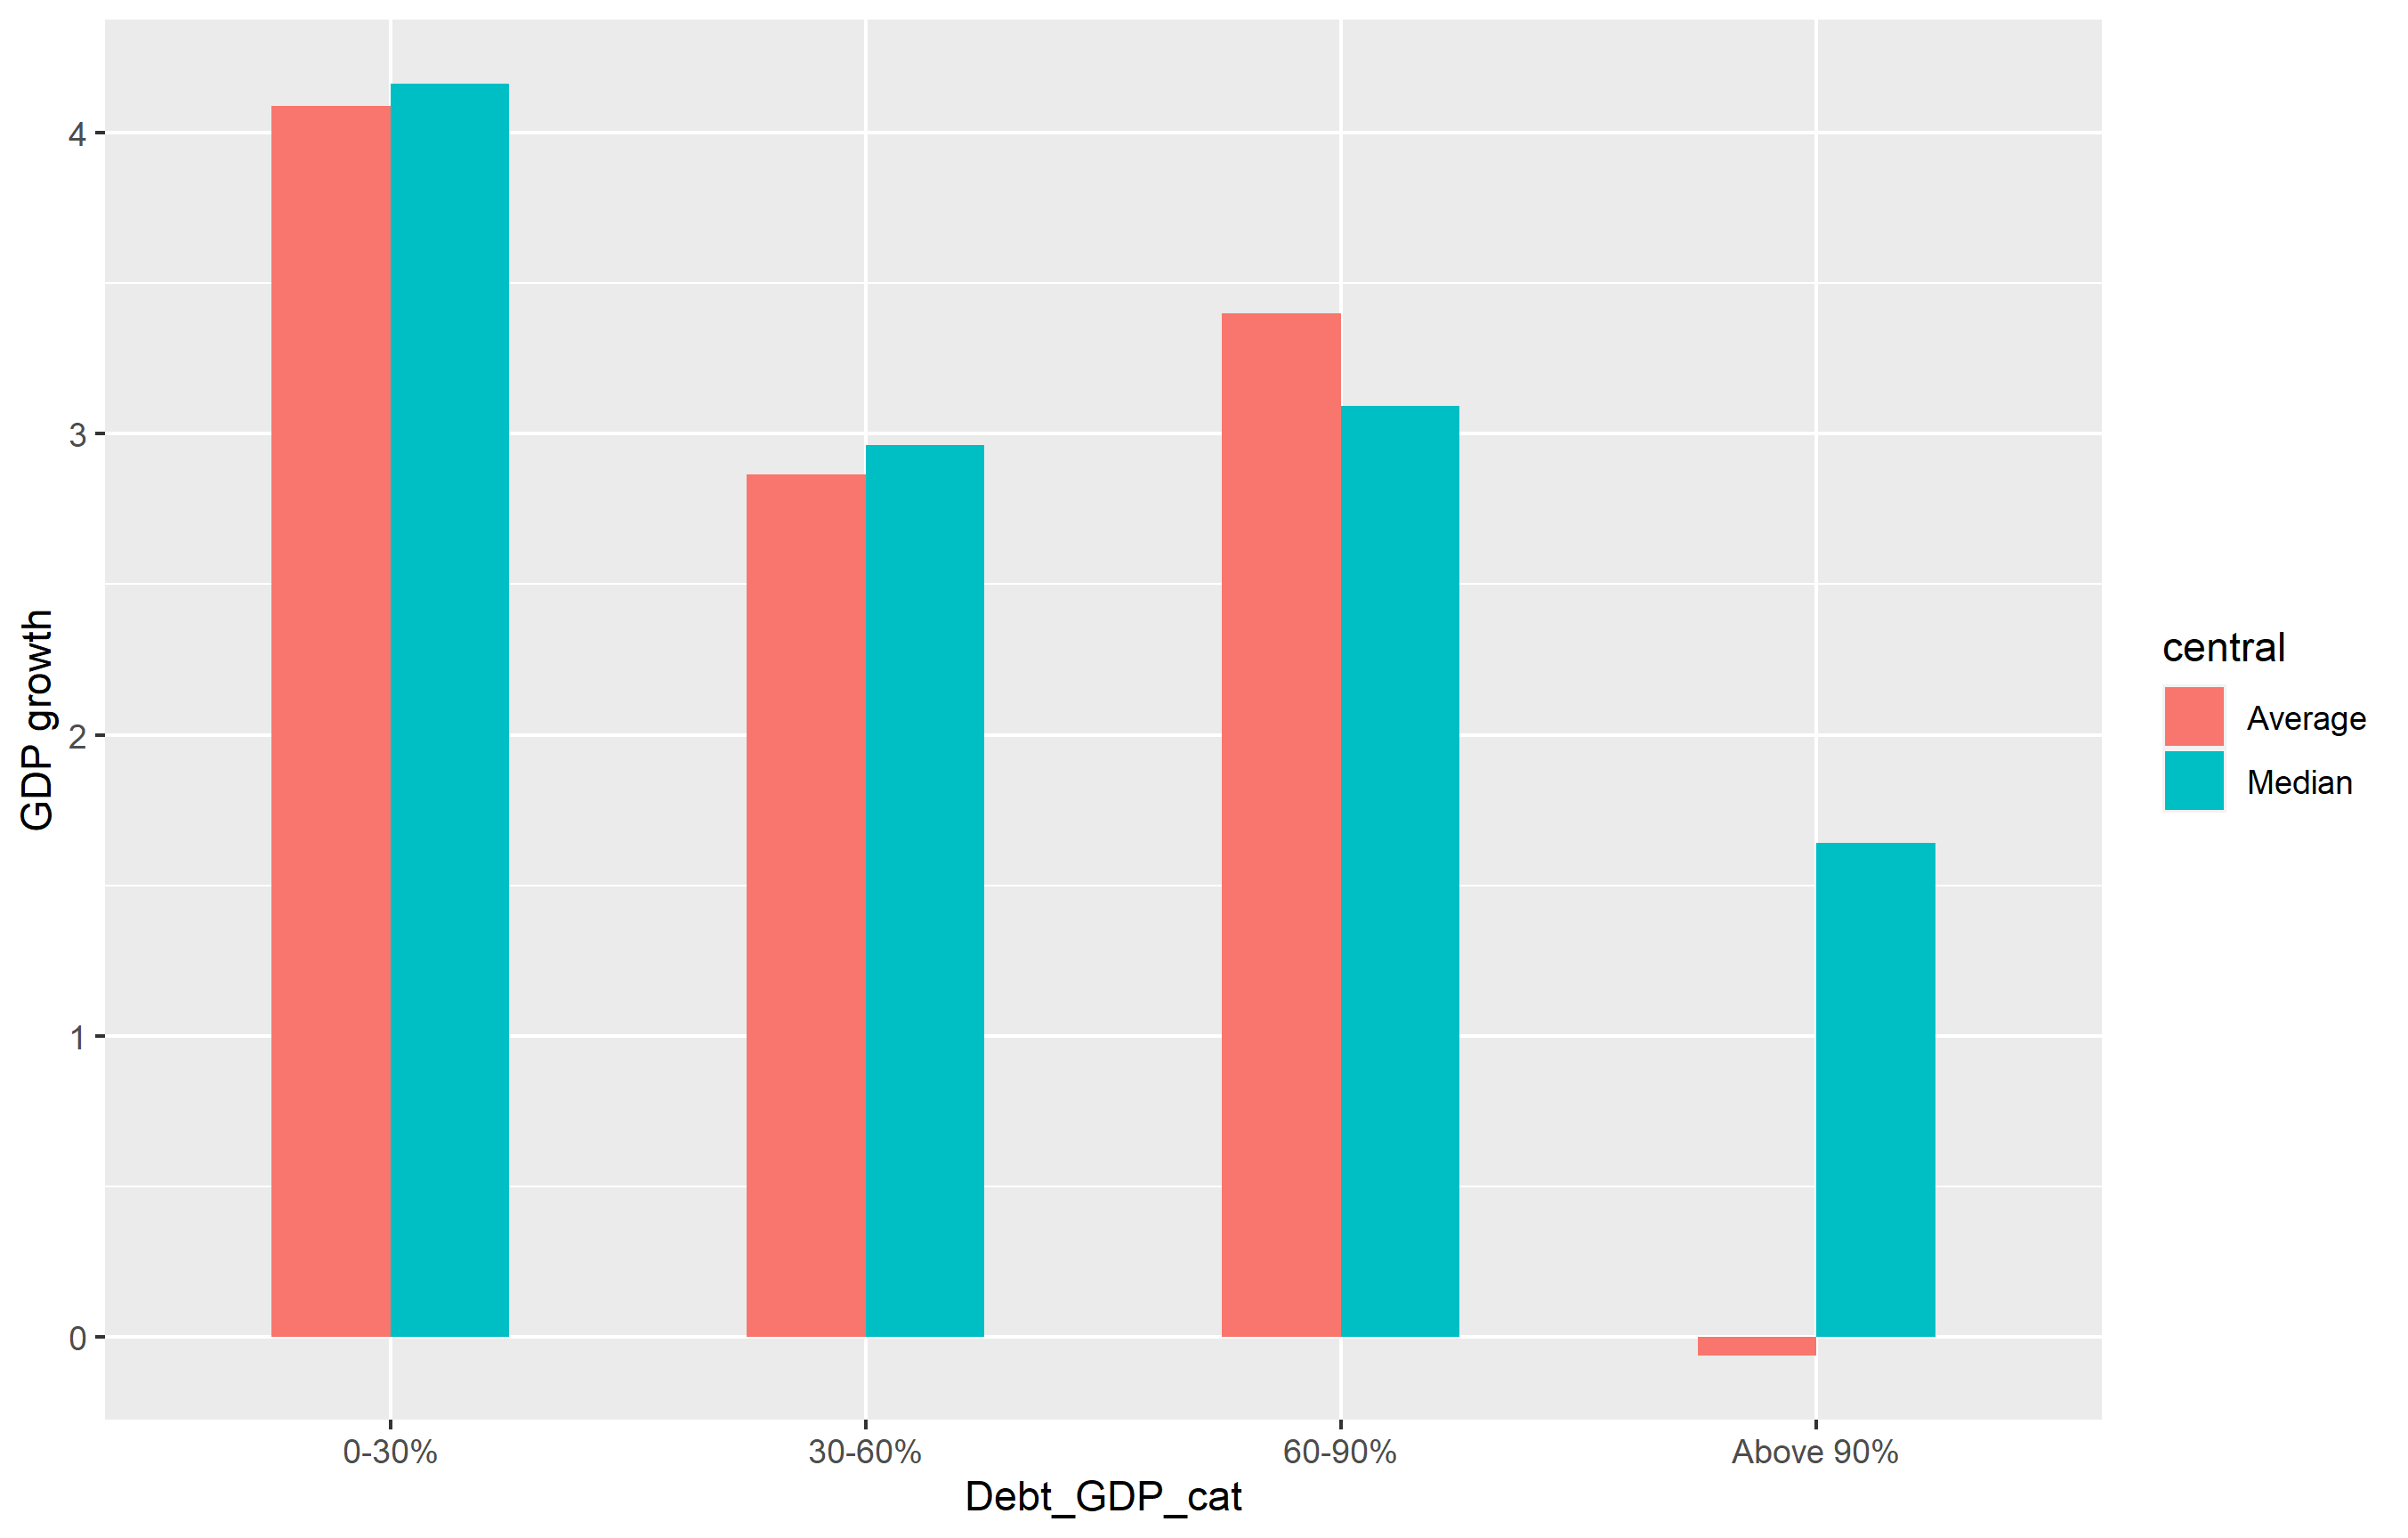
\includegraphics[width=0.75\linewidth]{F2} \caption{Figure 2 RR}\label{fig:pressure}
\end{figure}

\hypertarget{show-the-prevalence-of-the-four-public-debt-categories-for-the-sample-of-countries-over-time.show-the-real-gdp-growth-rate-for-the-sample-of-countries-over-time.-discuss-any-patterns-thatyou-observe.}{%
\subsection{2. Show the prevalence of the four public-debt categories
for the sample of countries over time.Show the real GDP growth rate for
the sample of countries over time. Discuss any patterns thatyou
observe.}\label{show-the-prevalence-of-the-four-public-debt-categories-for-the-sample-of-countries-over-time.show-the-real-gdp-growth-rate-for-the-sample-of-countries-over-time.-discuss-any-patterns-thatyou-observe.}}

\begin{Shaded}
\begin{Highlighting}[]
\KeywordTok{library}\NormalTok{(knitr)}
\KeywordTok{kable}\NormalTok{(prev_}\DecValTok{1}\NormalTok{)}
\end{Highlighting}
\end{Shaded}

\begin{longtable}[]{@{}lrrrr@{}}
\toprule
Country & 0-30\% & 30-60\% & 60-90\% & Above 90\%\tabularnewline
\midrule
\endhead
Australia & 37 & 13 & 9 & 5\tabularnewline
Austria & 34 & 25 & 0 & 0\tabularnewline
Belgium & 0 & 17 & 21 & 25\tabularnewline
Canada & 3 & 42 & 14 & 5\tabularnewline
Denmark & 23 & 16 & 17 & 0\tabularnewline
Finland & 44 & 16 & 4 & 0\tabularnewline
France & 24 & 20 & 10 & 0\tabularnewline
Germany & 48 & 11 & 0 & 0\tabularnewline
Greece & 13 & 5 & 3 & 19\tabularnewline
Ireland & 10 & 14 & 32 & 7\tabularnewline
Italy & 26 & 6 & 17 & 10\tabularnewline
Japan & 22 & 17 & 4 & 11\tabularnewline
Netherlands & 17 & 34 & 2 & 0\tabularnewline
New Zealand & 9 & 33 & 17 & 5\tabularnewline
Norway & 51 & 12 & 1 & 0\tabularnewline
Portugal & 42 & 9 & 7 & 0\tabularnewline
Spain & 5 & 36 & 1 & 0\tabularnewline
Sweden & 18 & 35 & 11 & 0\tabularnewline
UK & 0 & 38 & 6 & 19\tabularnewline
US & 0 & 37 & 23 & 4\tabularnewline
\bottomrule
\end{longtable}

\begin{Shaded}
\begin{Highlighting}[]
\KeywordTok{library}\NormalTok{(knitr)}
\KeywordTok{kable}\NormalTok{(prev_}\DecValTok{2}\NormalTok{)}
\end{Highlighting}
\end{Shaded}

\begin{longtable}[]{@{}rrrr@{}}
\toprule
0-30\% & 30-60\% & 60-90\% & Above 90\%\tabularnewline
\midrule
\endhead
426 & 436 & 199 & 110\tabularnewline
\bottomrule
\end{longtable}

Prevalence of Real GDP Growth

\begin{Shaded}
\begin{Highlighting}[]
\KeywordTok{library}\NormalTok{(knitr)}
\KeywordTok{kable}\NormalTok{(prevGDP)}
\end{Highlighting}
\end{Shaded}

\begin{longtable}[]{@{}lrrrrrrr@{}}
\toprule
Country & 1946-1950 & 1951-1960 & 1961-1970 & 1971-1980 & 1981-1990 &
1991-2000 & 2000-2010\tabularnewline
\midrule
\endhead
Australia & 3.7742505 & 4.057079 & 5.286783 & 3.310568 & 3.246736 &
3.441959 & 2.8755253\tabularnewline
Austria & 19.5468645 & 6.028140 & 4.720503 & 3.644882 & 2.316075 &
2.557066 & 1.7560900\tabularnewline
Belgium & 7.7478861 & 2.641468 & 5.127077 & 3.573654 & 2.057382 &
2.349175 & 1.2918860\tabularnewline
Canada & 2.9566400 & 4.620591 & 5.079180 & 4.273472 & 2.535731 &
3.710663 & 1.8610558\tabularnewline
Denmark & 7.9458545 & 3.163720 & 4.499750 & 1.589972 & 2.094581 &
2.605949 & 0.8501989\tabularnewline
Finland & 5.6593573 & 4.975873 & 4.831884 & 3.481533 & 3.034762 &
2.070023 & 1.8182061\tabularnewline
France & 7.4940048 & 4.578134 & 5.579828 & 3.908958 & 2.535731 &
3.710663 & 1.8610558\tabularnewline
Germany & NA & 7.739168 & 4.219219 & 2.756779 & 2.315392 & 2.079083 &
0.4975409\tabularnewline
Greece & NA & NA & 7.954927 & 4.674873 & 0.710200 & 2.355700 &
3.5272222\tabularnewline
Ireland & 3.2026001 & 1.739933 & 4.215289 & 4.736466 & 2.870000 &
7.110000 & 3.1444444\tabularnewline
Italy & NA & 6.060585 & 5.815893 & 3.128034 & 2.407300 & 1.592300 &
0.2064444\tabularnewline
Japan & NA & 7.906044 & 9.139496 & 4.601107 & 4.643919 & 1.193078 &
0.5378570\tabularnewline
Netherlands & NA & 3.954550 & 5.085018 & 2.931332 & 2.254174 & 3.067691
& 1.2723563\tabularnewline
New Zealand & 7.0369371 & 3.484836 & 3.581376 & 2.239731 & 1.723000 &
2.877800 & 2.4655556\tabularnewline
Norway & 7.6505874 & 3.836354 & 4.197120 & 4.710583 & 2.535731 &
3.710663 & 1.8610558\tabularnewline
Portugal & 2.8372935 & 4.762352 & 6.382186 & 4.819081 & 2.535731 &
3.710663 & 1.8610558\tabularnewline
Spain & 1.6924847 & 5.737635 & NA & NA & 2.981895 & 2.907287 &
2.3332958\tabularnewline
Sweden & 6.1217601 & 3.620328 & 5.274890 & 1.967190 & 2.203565 &
2.026641 & 1.6255954\tabularnewline
UK & 1.1371502 & 2.670354 & 2.832633 & 1.984710 & 2.733149 & 2.547979 &
2.3448646\tabularnewline
US & 0.1576796 & 3.547241 & 4.215048 & 3.209143 & 3.266144 & 3.411775 &
1.6148628\tabularnewline
\bottomrule
\end{longtable}

\hypertarget{replication-of-figures-1-2-and-4-of-herndon-et-al.}{%
\subsection{3. Replication of figures 1, 2 and 4 of Herndon et
al.~}\label{replication-of-figures-1-2-and-4-of-herndon-et-al.}}

Figure 1 Herndon

\begin{figure}
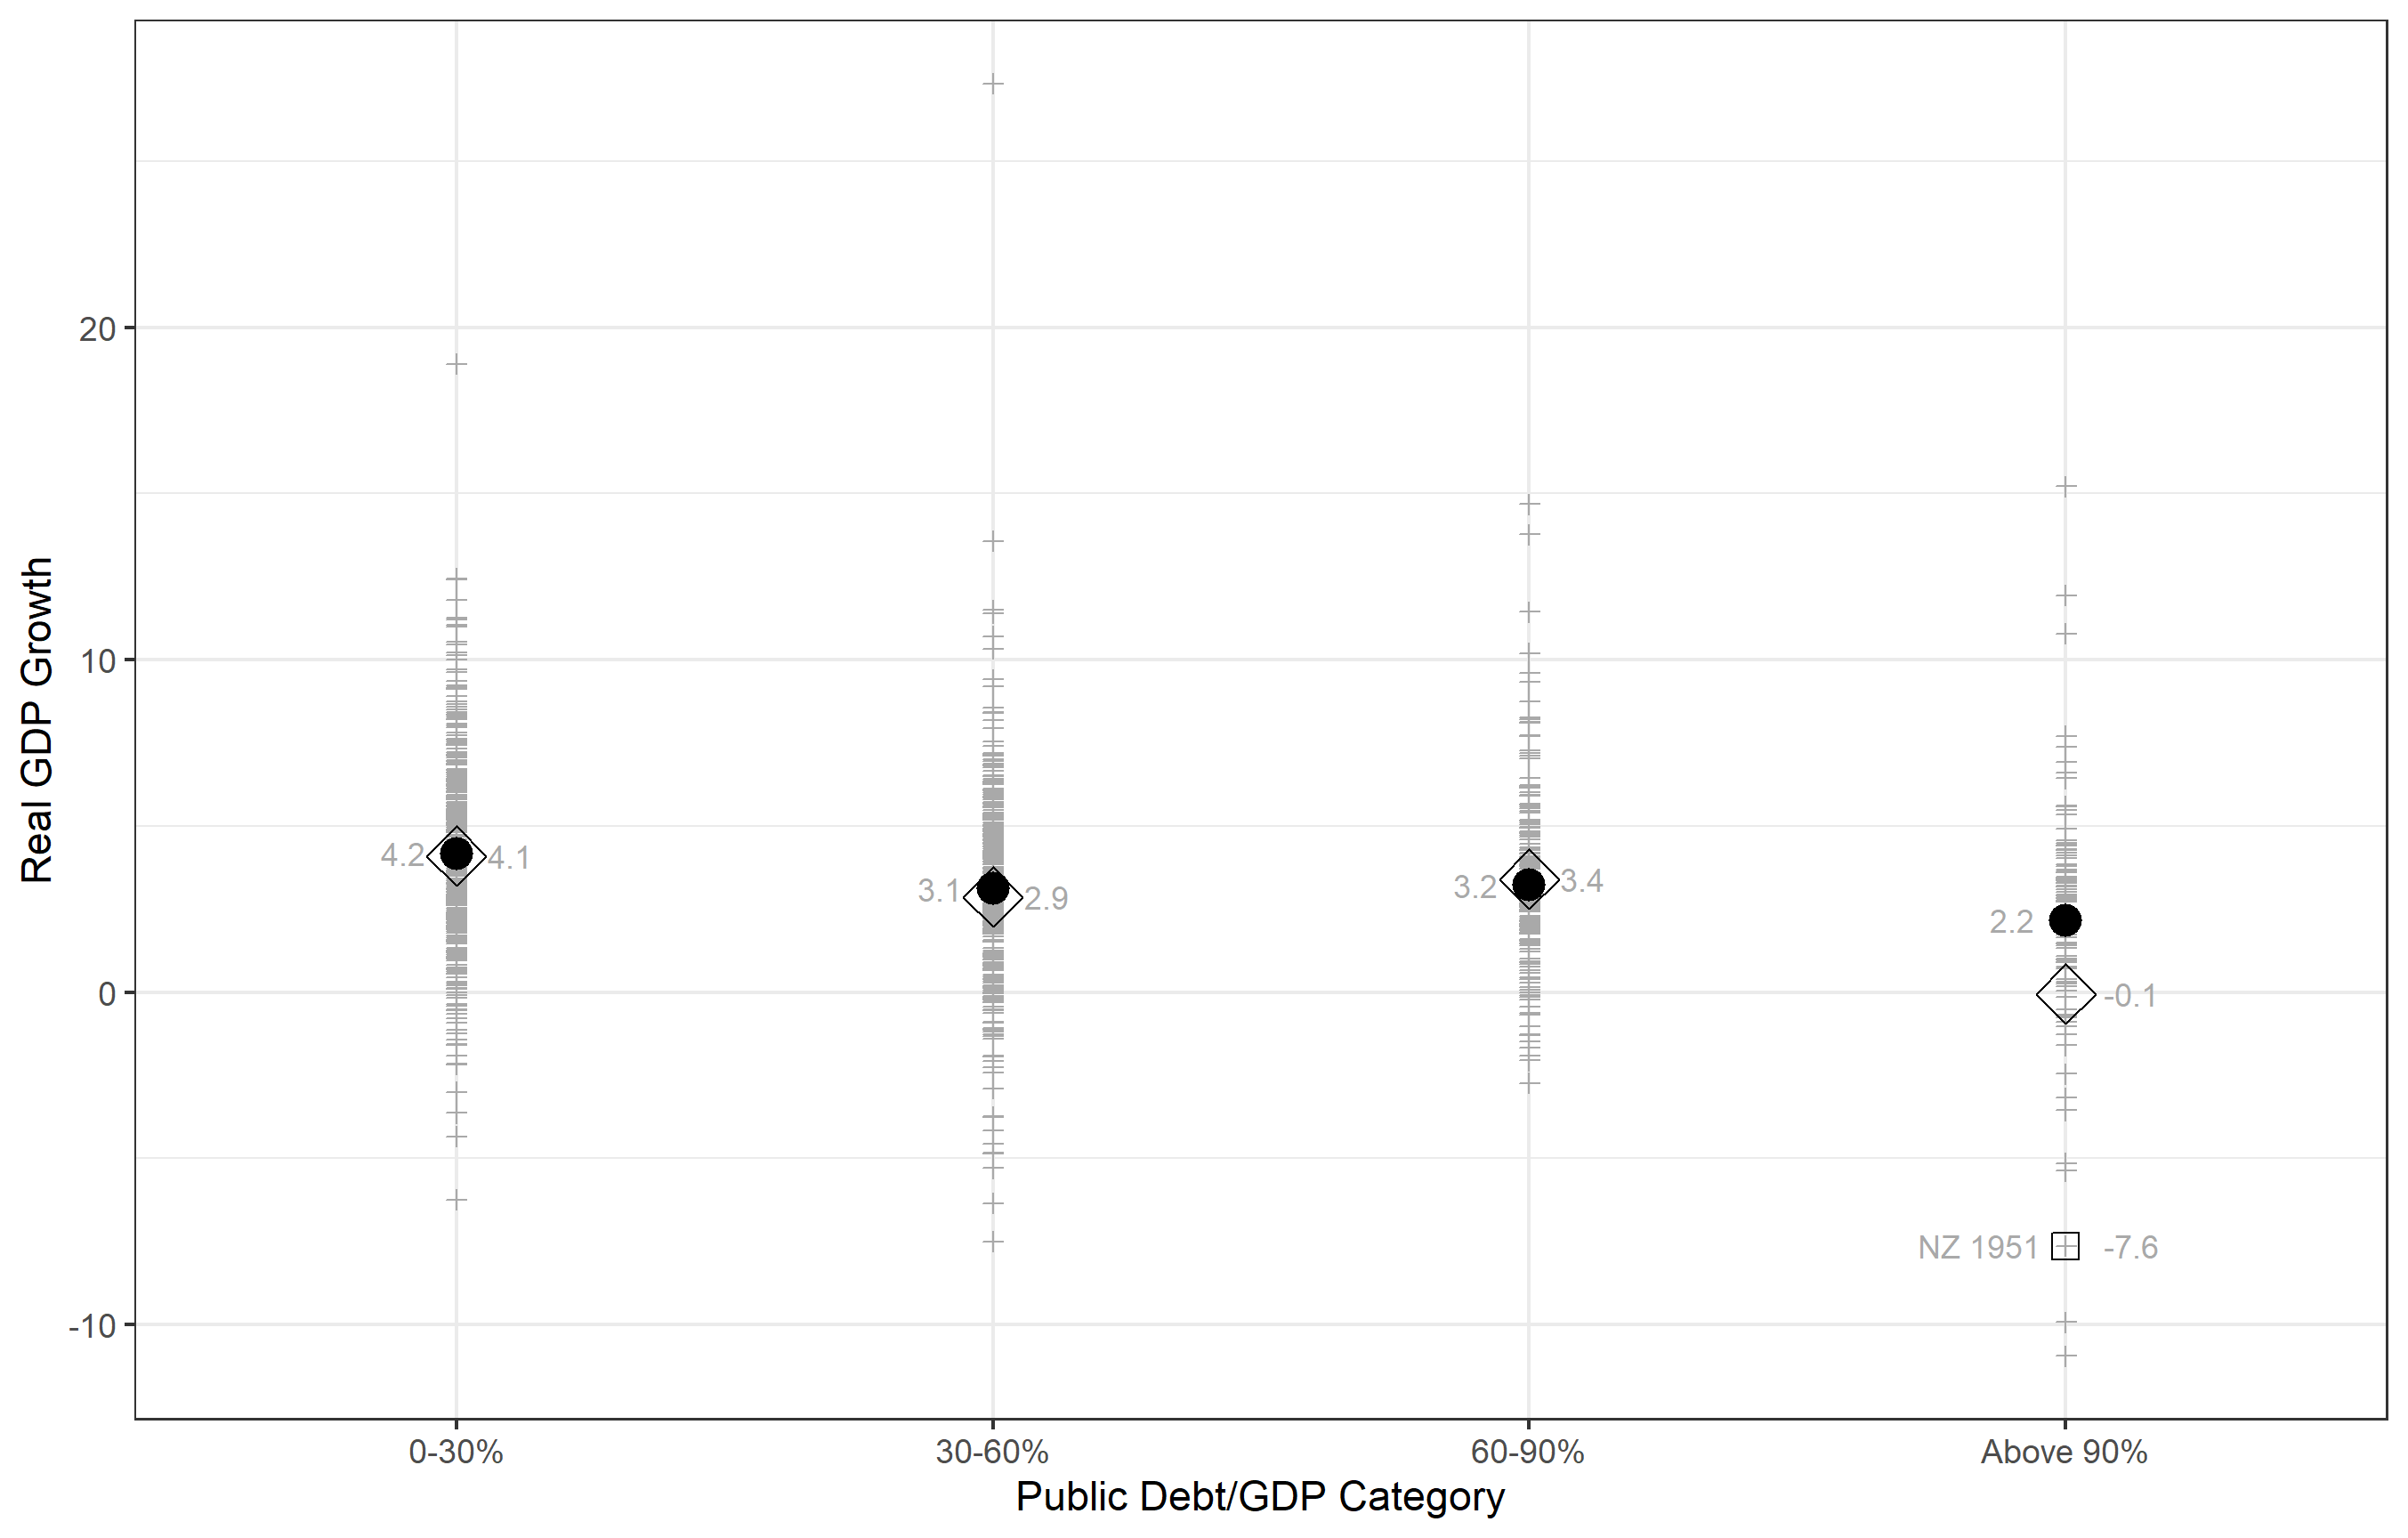
\includegraphics[width=0.75\linewidth]{Figure_1_Herndon} \caption{Figure 1 Herndon et al.}\label{fig:unnamed-chunk-14}
\end{figure}

Figure 2 Herndon

\begin{figure}
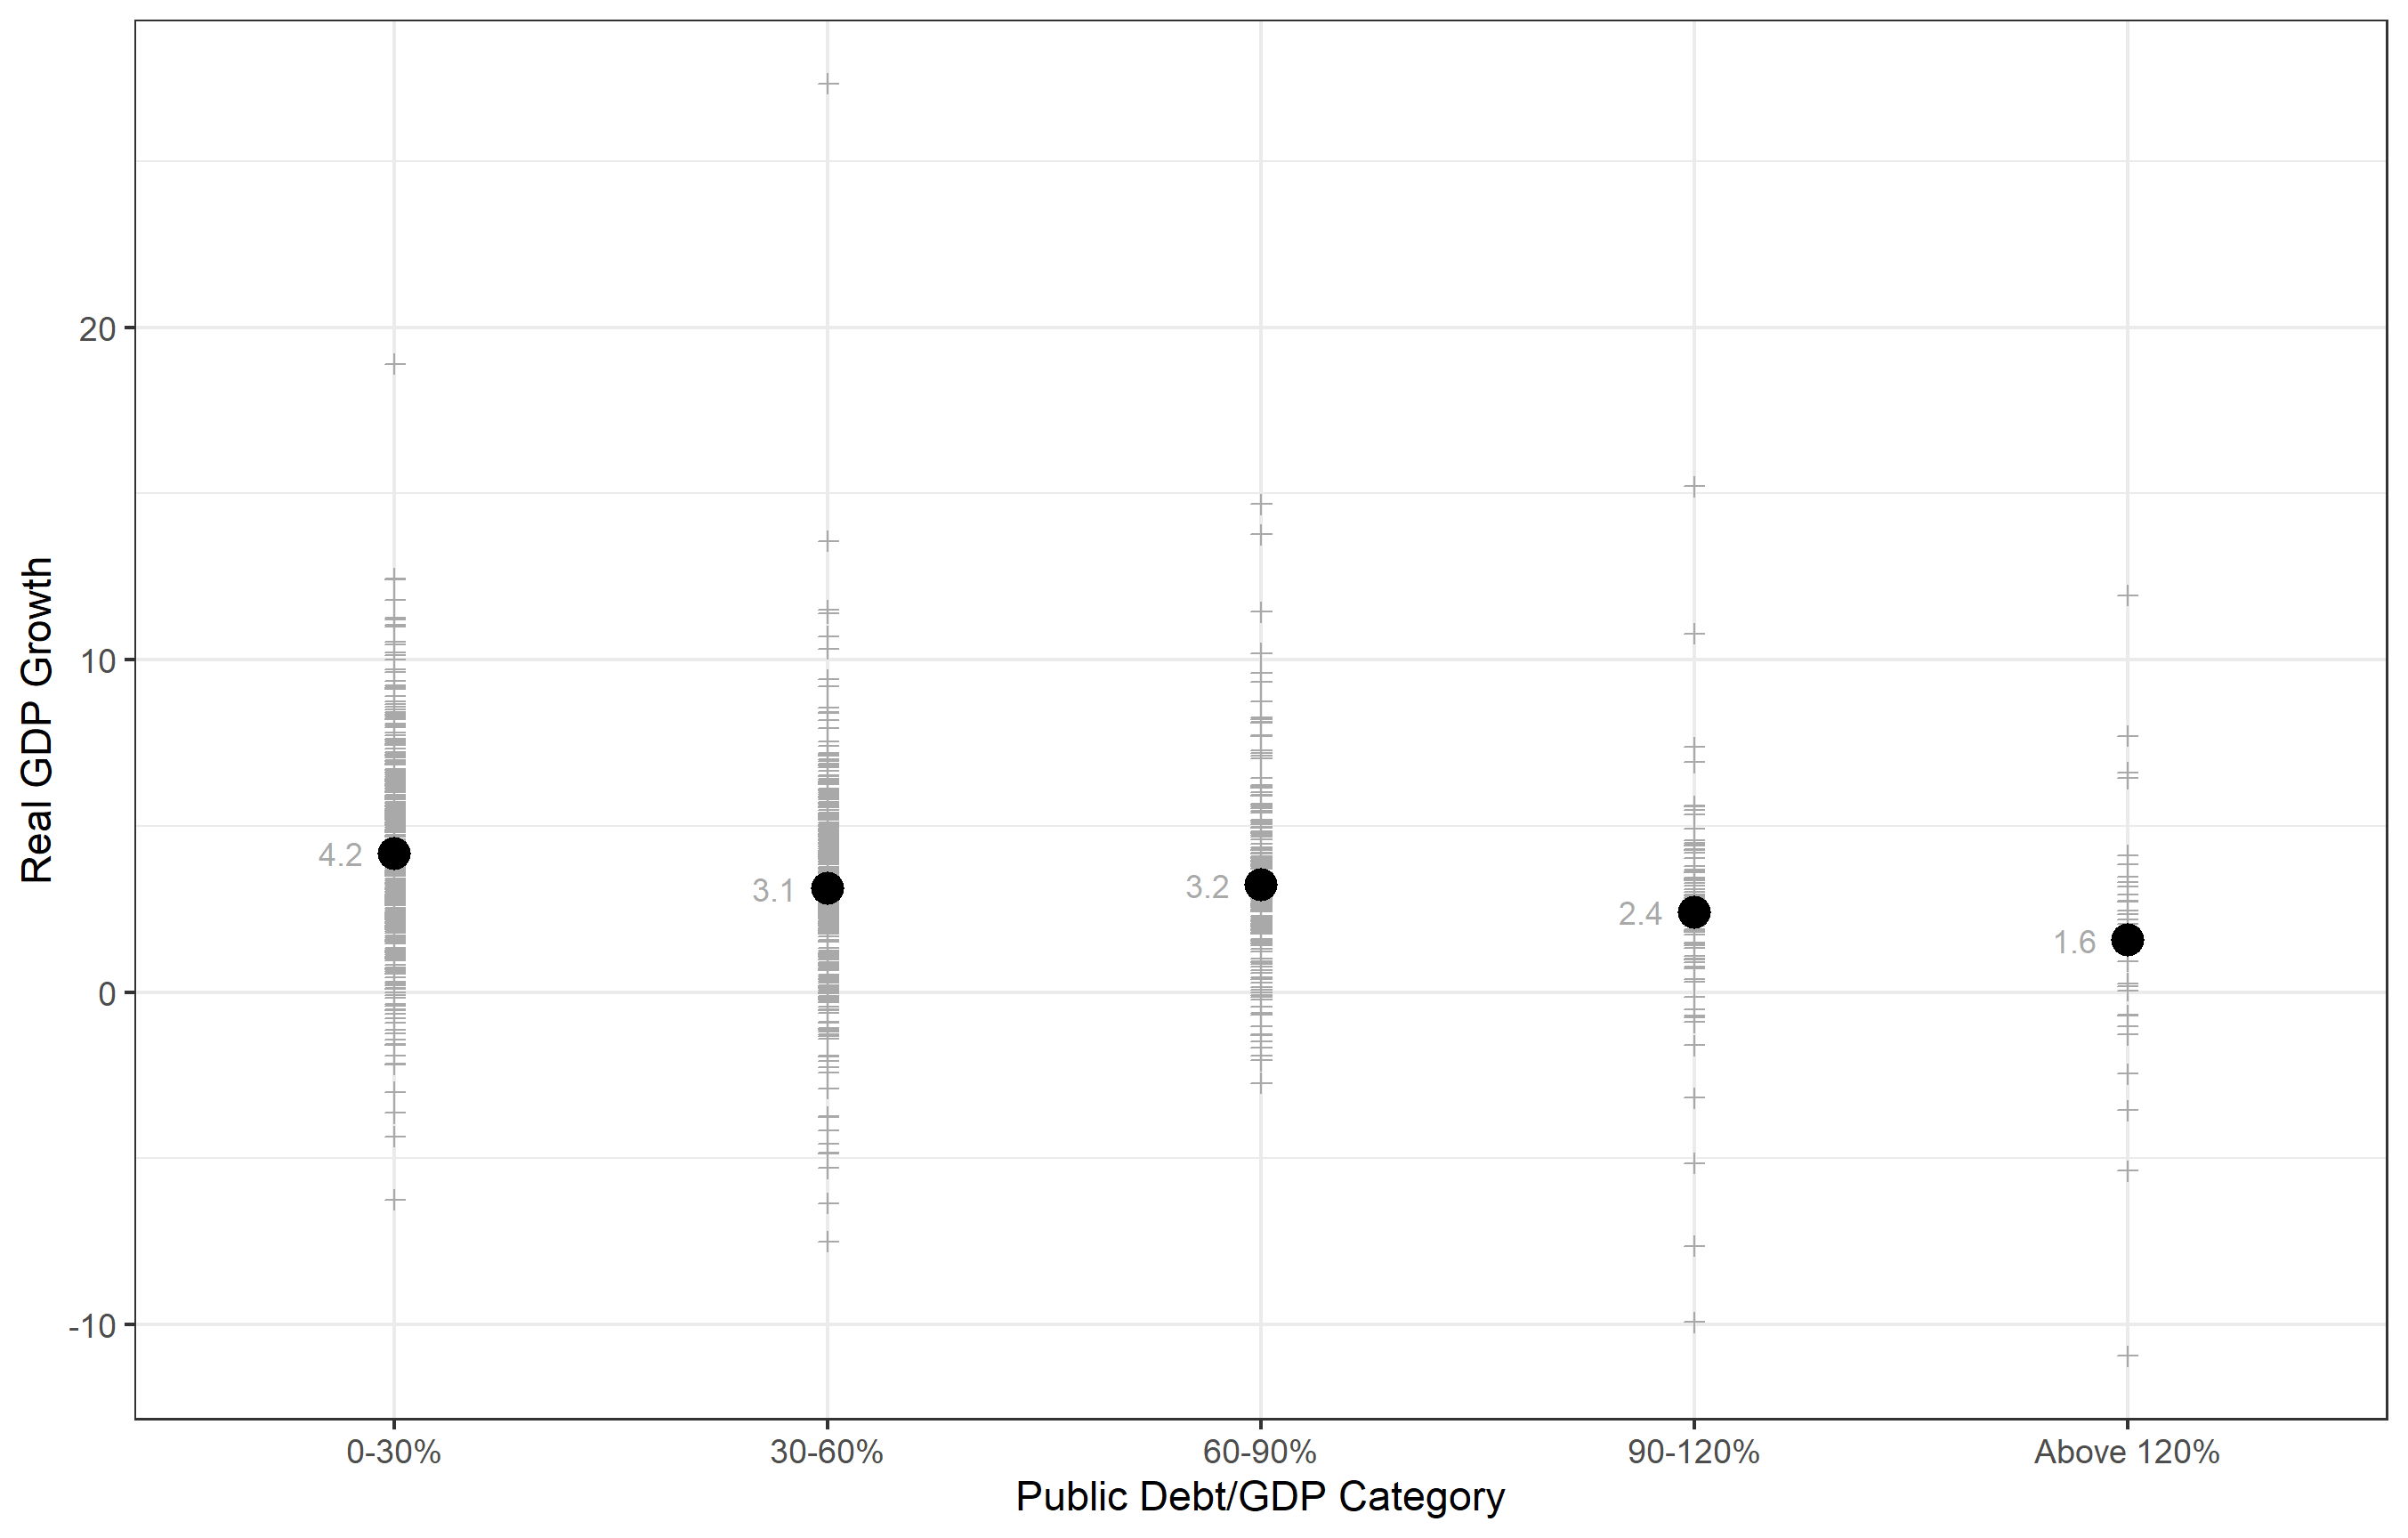
\includegraphics[width=0.75\linewidth]{Figure_2_Herndon} \caption{Figure 2 Herndon et al.}\label{fig:unnamed-chunk-15}
\end{figure}

Figure 4 Herndon

\begin{figure}
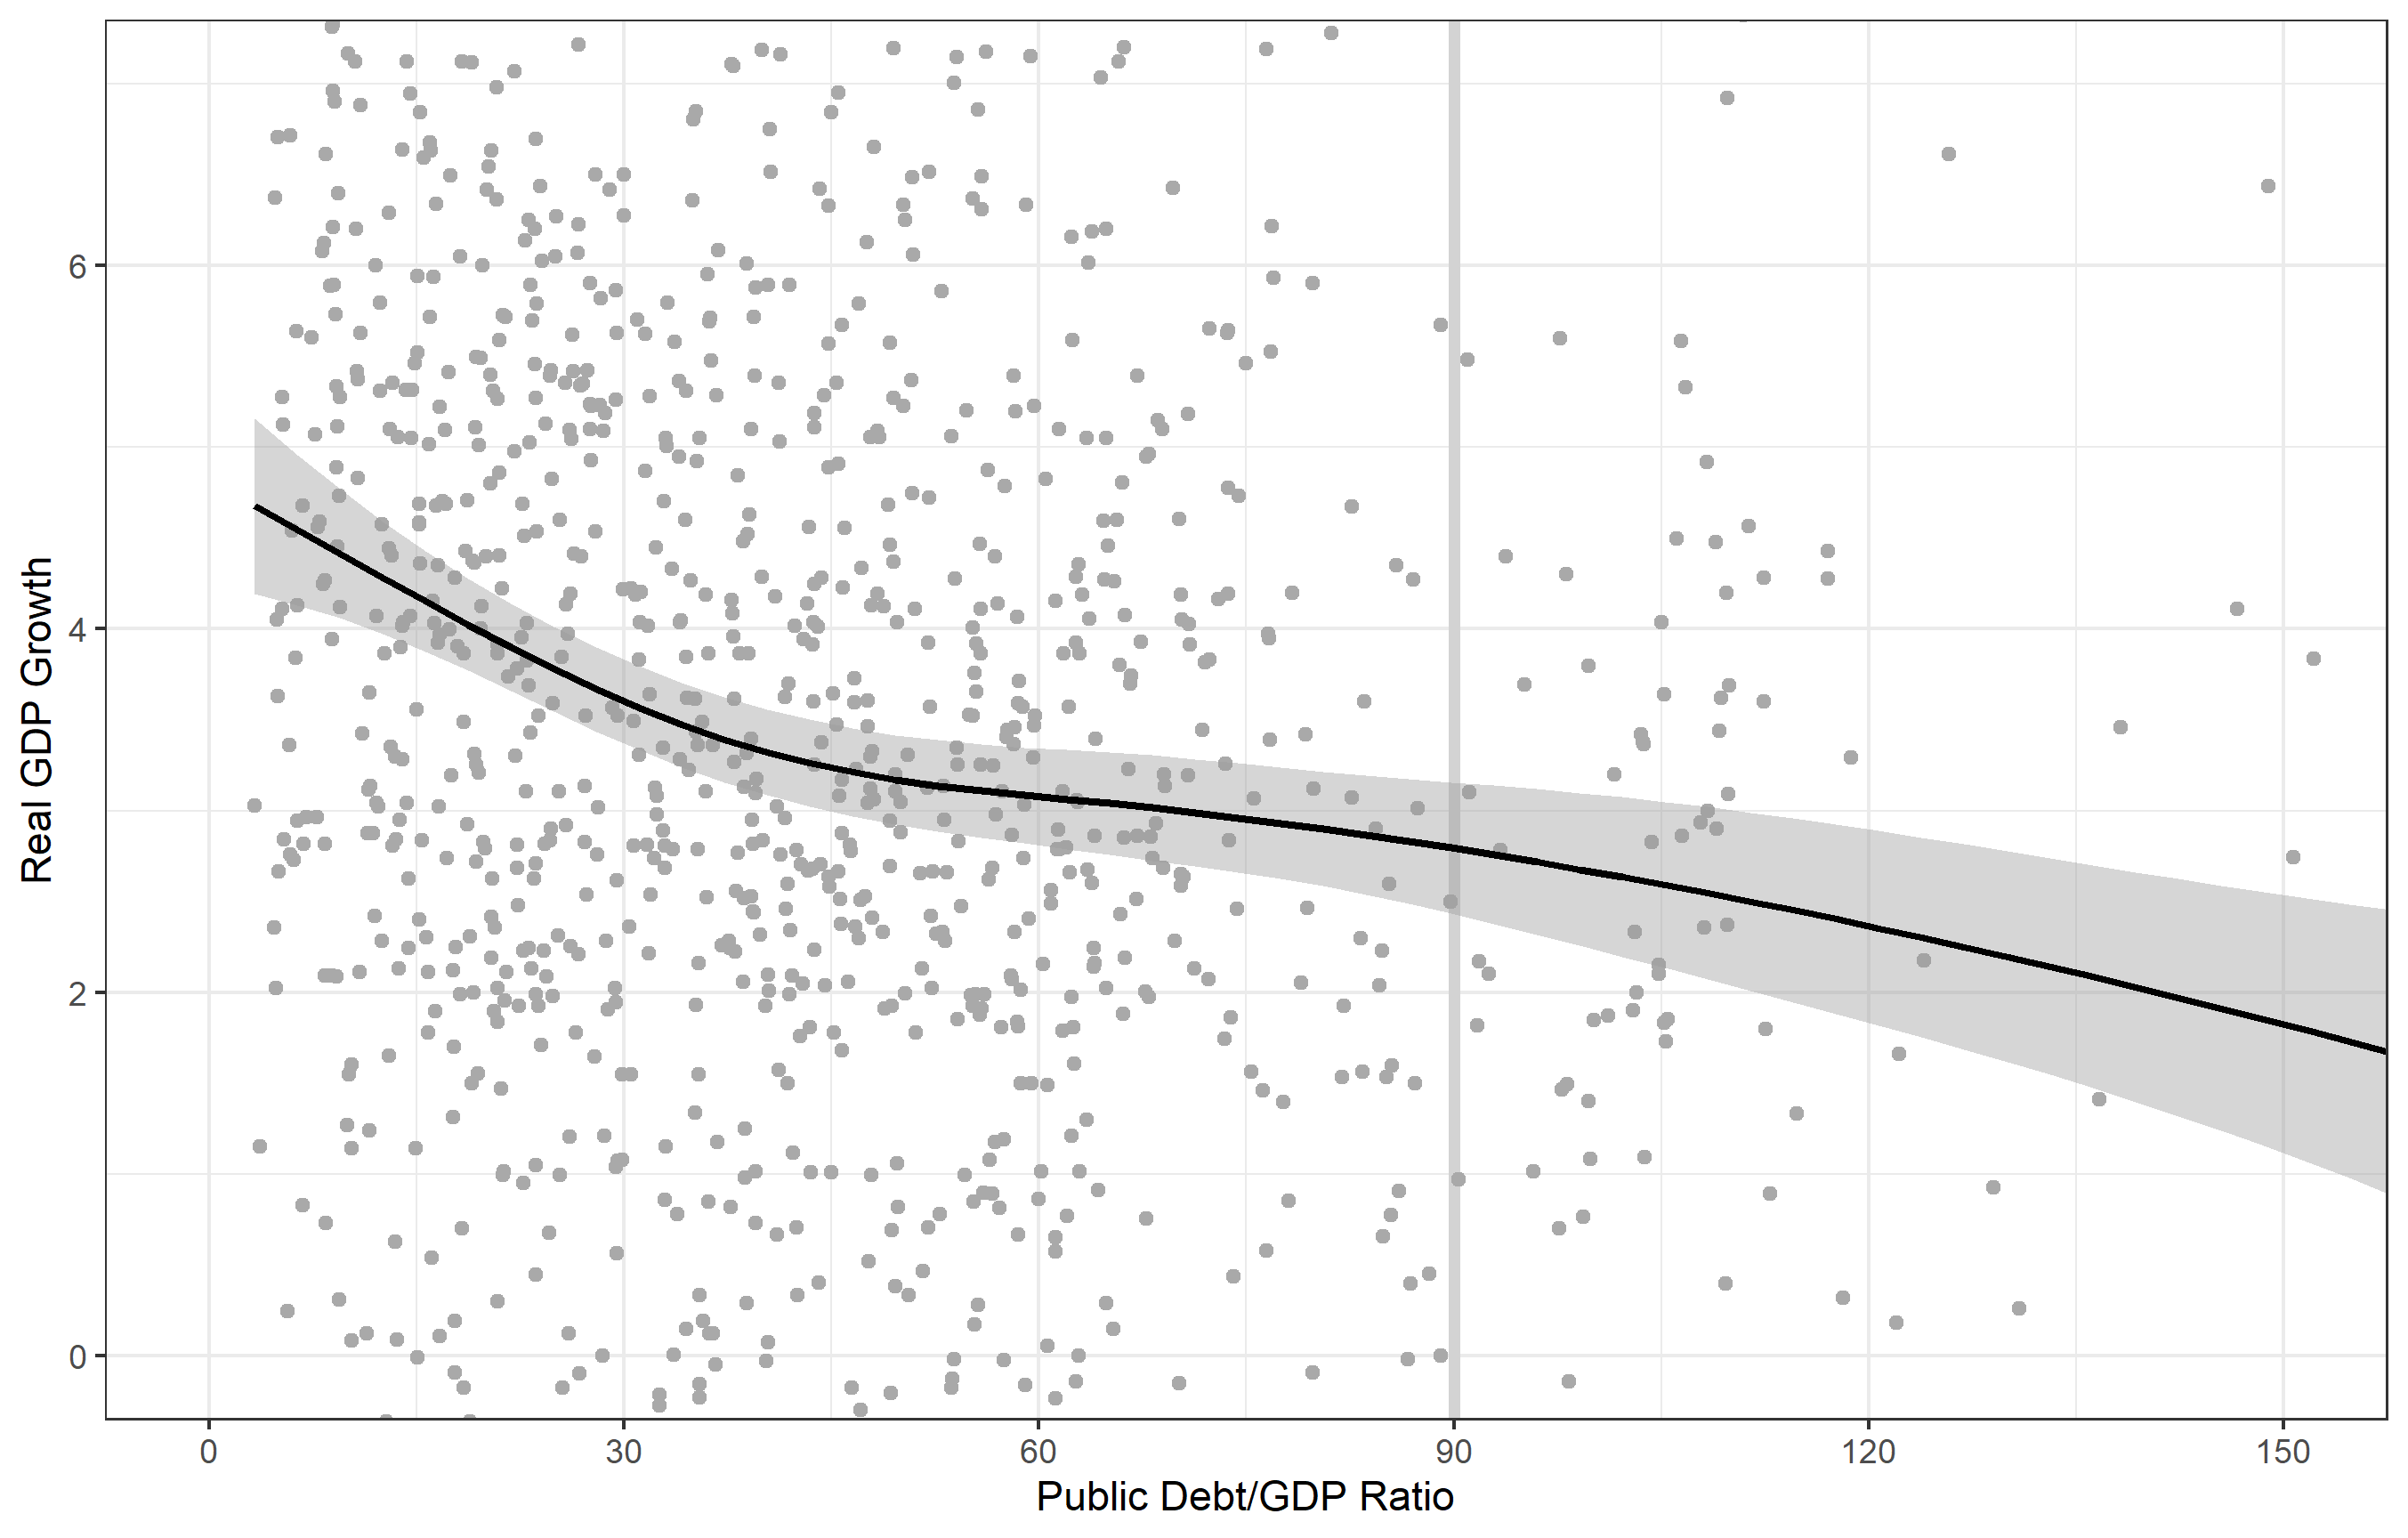
\includegraphics[width=0.75\linewidth]{Figure_4_Herndon} \caption{Figure 4 Herndon et al.}\label{fig:unnamed-chunk-16}
\end{figure}

\hypertarget{reorganization-in-a-meaningful-way}{%
\subsubsection{Reorganization in a meaningful
way}\label{reorganization-in-a-meaningful-way}}

\begin{figure}
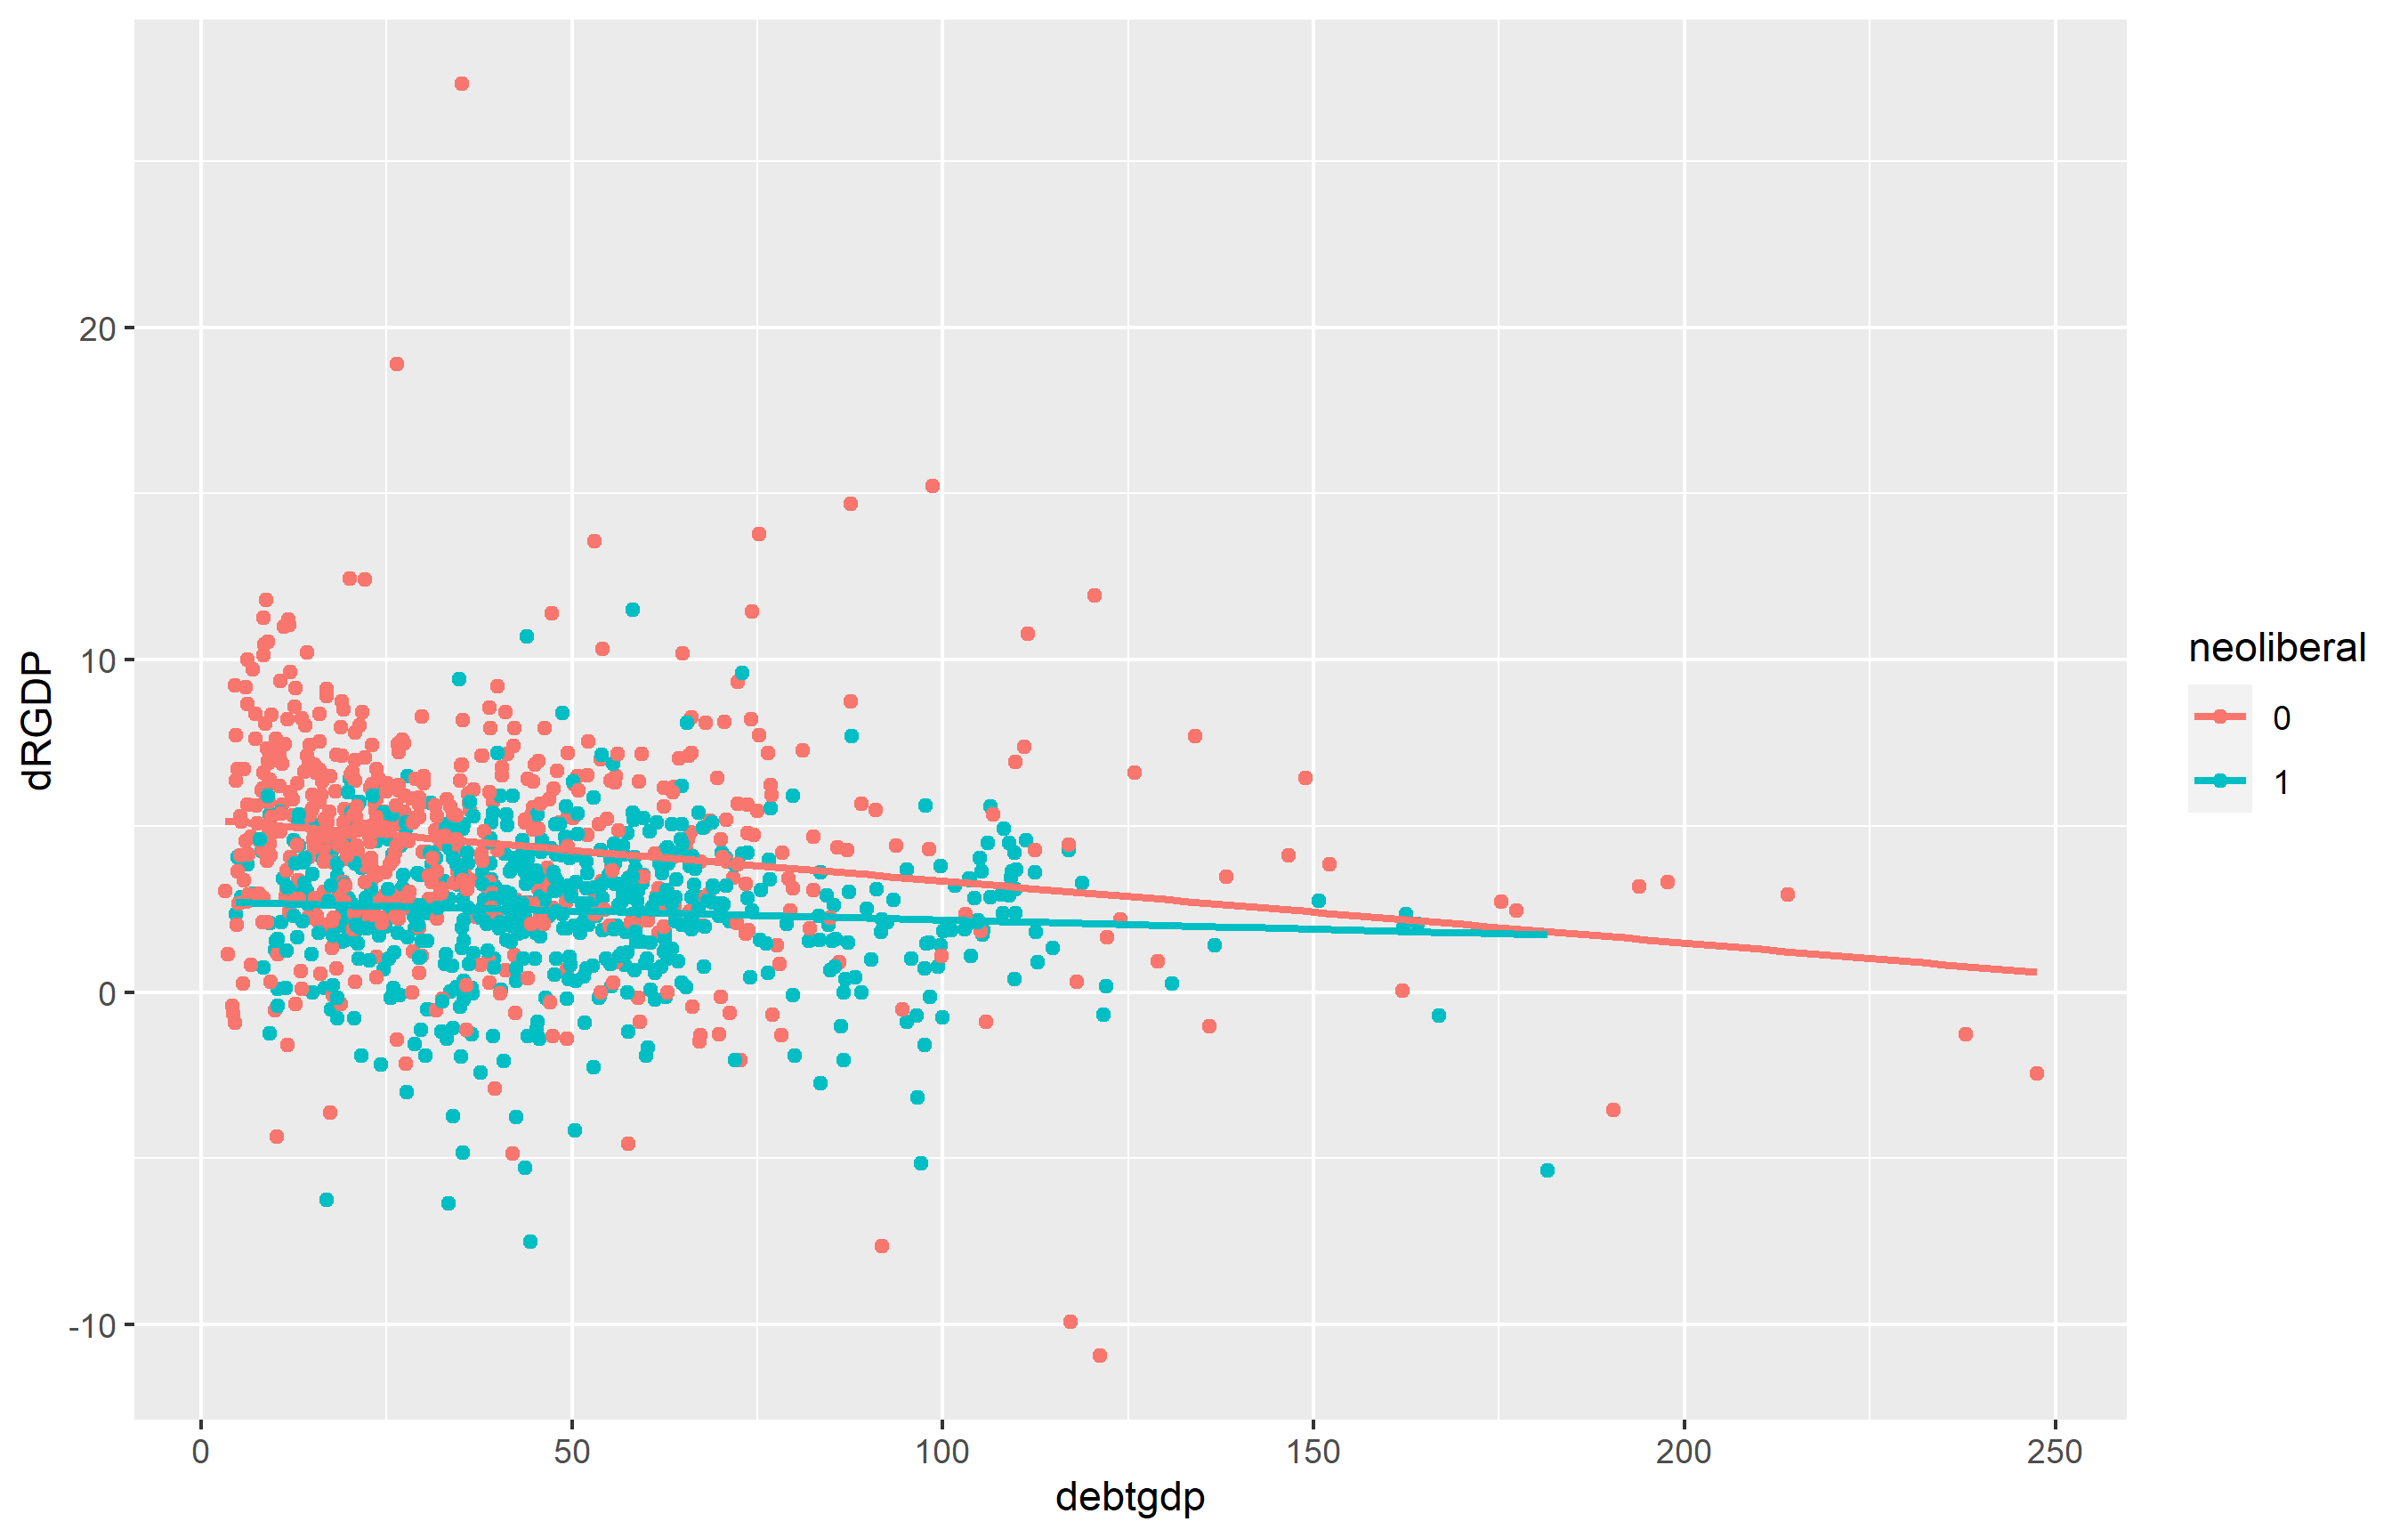
\includegraphics[width=0.75\linewidth]{gn} \caption{Before and After 1979}\label{fig:unnamed-chunk-17}
\end{figure}

\begin{figure}
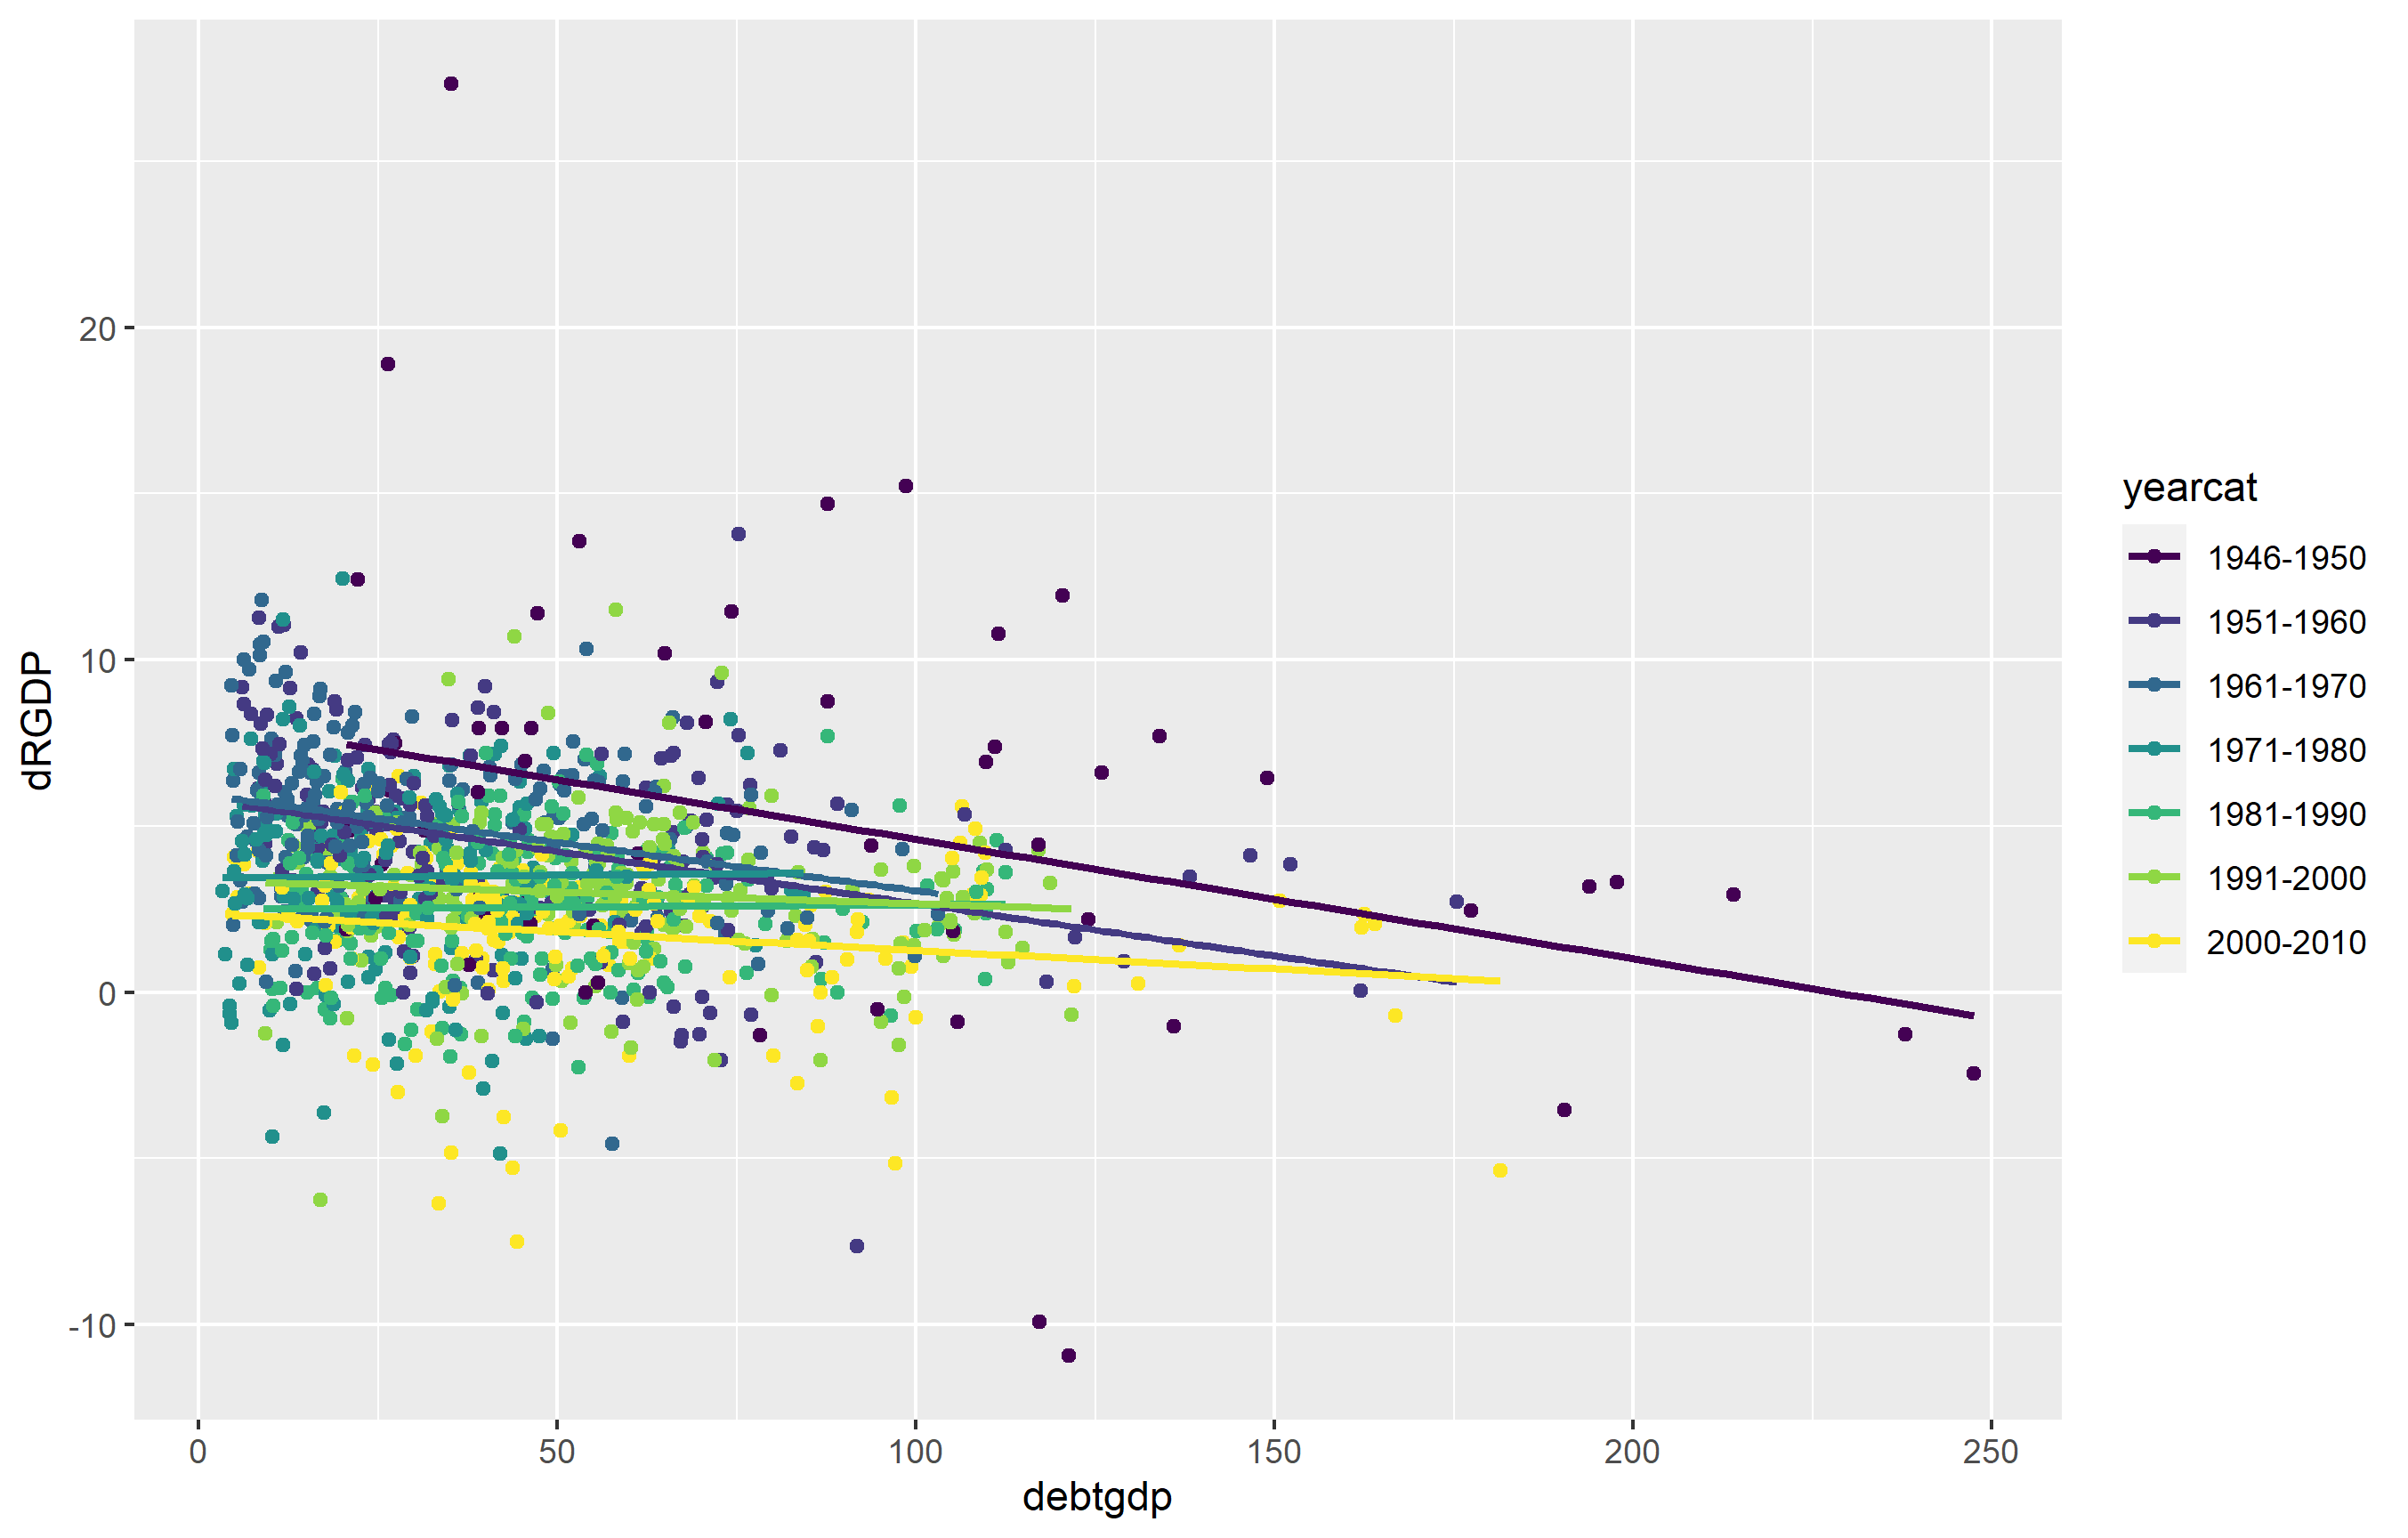
\includegraphics[width=0.75\linewidth]{gycat} \caption{Before and After 1979}\label{fig:unnamed-chunk-18}
\end{figure}

\end{document}
